\documentclass[11pt]{article}

\newcommand{\cnum}{ECE M146}
\newcommand{\ced}{Spring 2023}
\newcommand{\ctitle}[4]{\title{\vspace{-0.5in}\cnum, \ced\\Homework Set #1: #2}\author{\vspace{-0.35in}\\Name: #3, UID: #4}}
\usepackage{enumitem}
\newcommand{\solution}[1]{{{\color{blue}{\bf Solution:} {#1}}}}
\usepackage[usenames,dvipsnames,svgnames,table,hyperref]{xcolor}
\usepackage{amsmath, amsfonts}
\usepackage{graphicx} % Required for inserting images
\usepackage{float}
\usepackage{listings}
\usepackage{xcolor}
\usepackage{hyperref}

\renewcommand*{\theenumi}{\alph{enumi}}
\renewcommand*\labelenumi{(\theenumi)}
\renewcommand*{\theenumii}{\roman{enumii}}
\renewcommand*\labelenumii{\theenumii.}

\definecolor{codegreen}{rgb}{0,0.6,0}
\definecolor{codegray}{rgb}{0.5,0.5,0.5}
\definecolor{codepurple}{rgb}{0.58,0,0.82}
\definecolor{backcolour}{rgb}{0.95,0.95,0.92}

\lstdefinestyle{mystyle}{
    backgroundcolor=\color{backcolour},
    commentstyle=\color{codegreen},
    keywordstyle=\color{magenta},
    numberstyle=\tiny\color{codegray},
    stringstyle=\color{codepurple},
    basicstyle=\ttfamily\footnotesize,
    breakatwhitespace=false,
    breaklines=true,
    captionpos=b,
    keepspaces=true,
    numbers=left,
    numbersep=5pt,
    showspaces=false,
    showstringspaces=false,
    showtabs=false,
    tabsize=2
}


\begin{document}
\ctitle{\#1}{}{Asher Christian}{006-150-286}
\date{}
\maketitle
\vspace{-0.75in}
\section{Problem 1}
\solution{
    \begin{enumerate}
        \item No the data is not linearly separable, the algorithm will not converge if we run it several times over the same sequence. This can be seen by visualizing the data.
            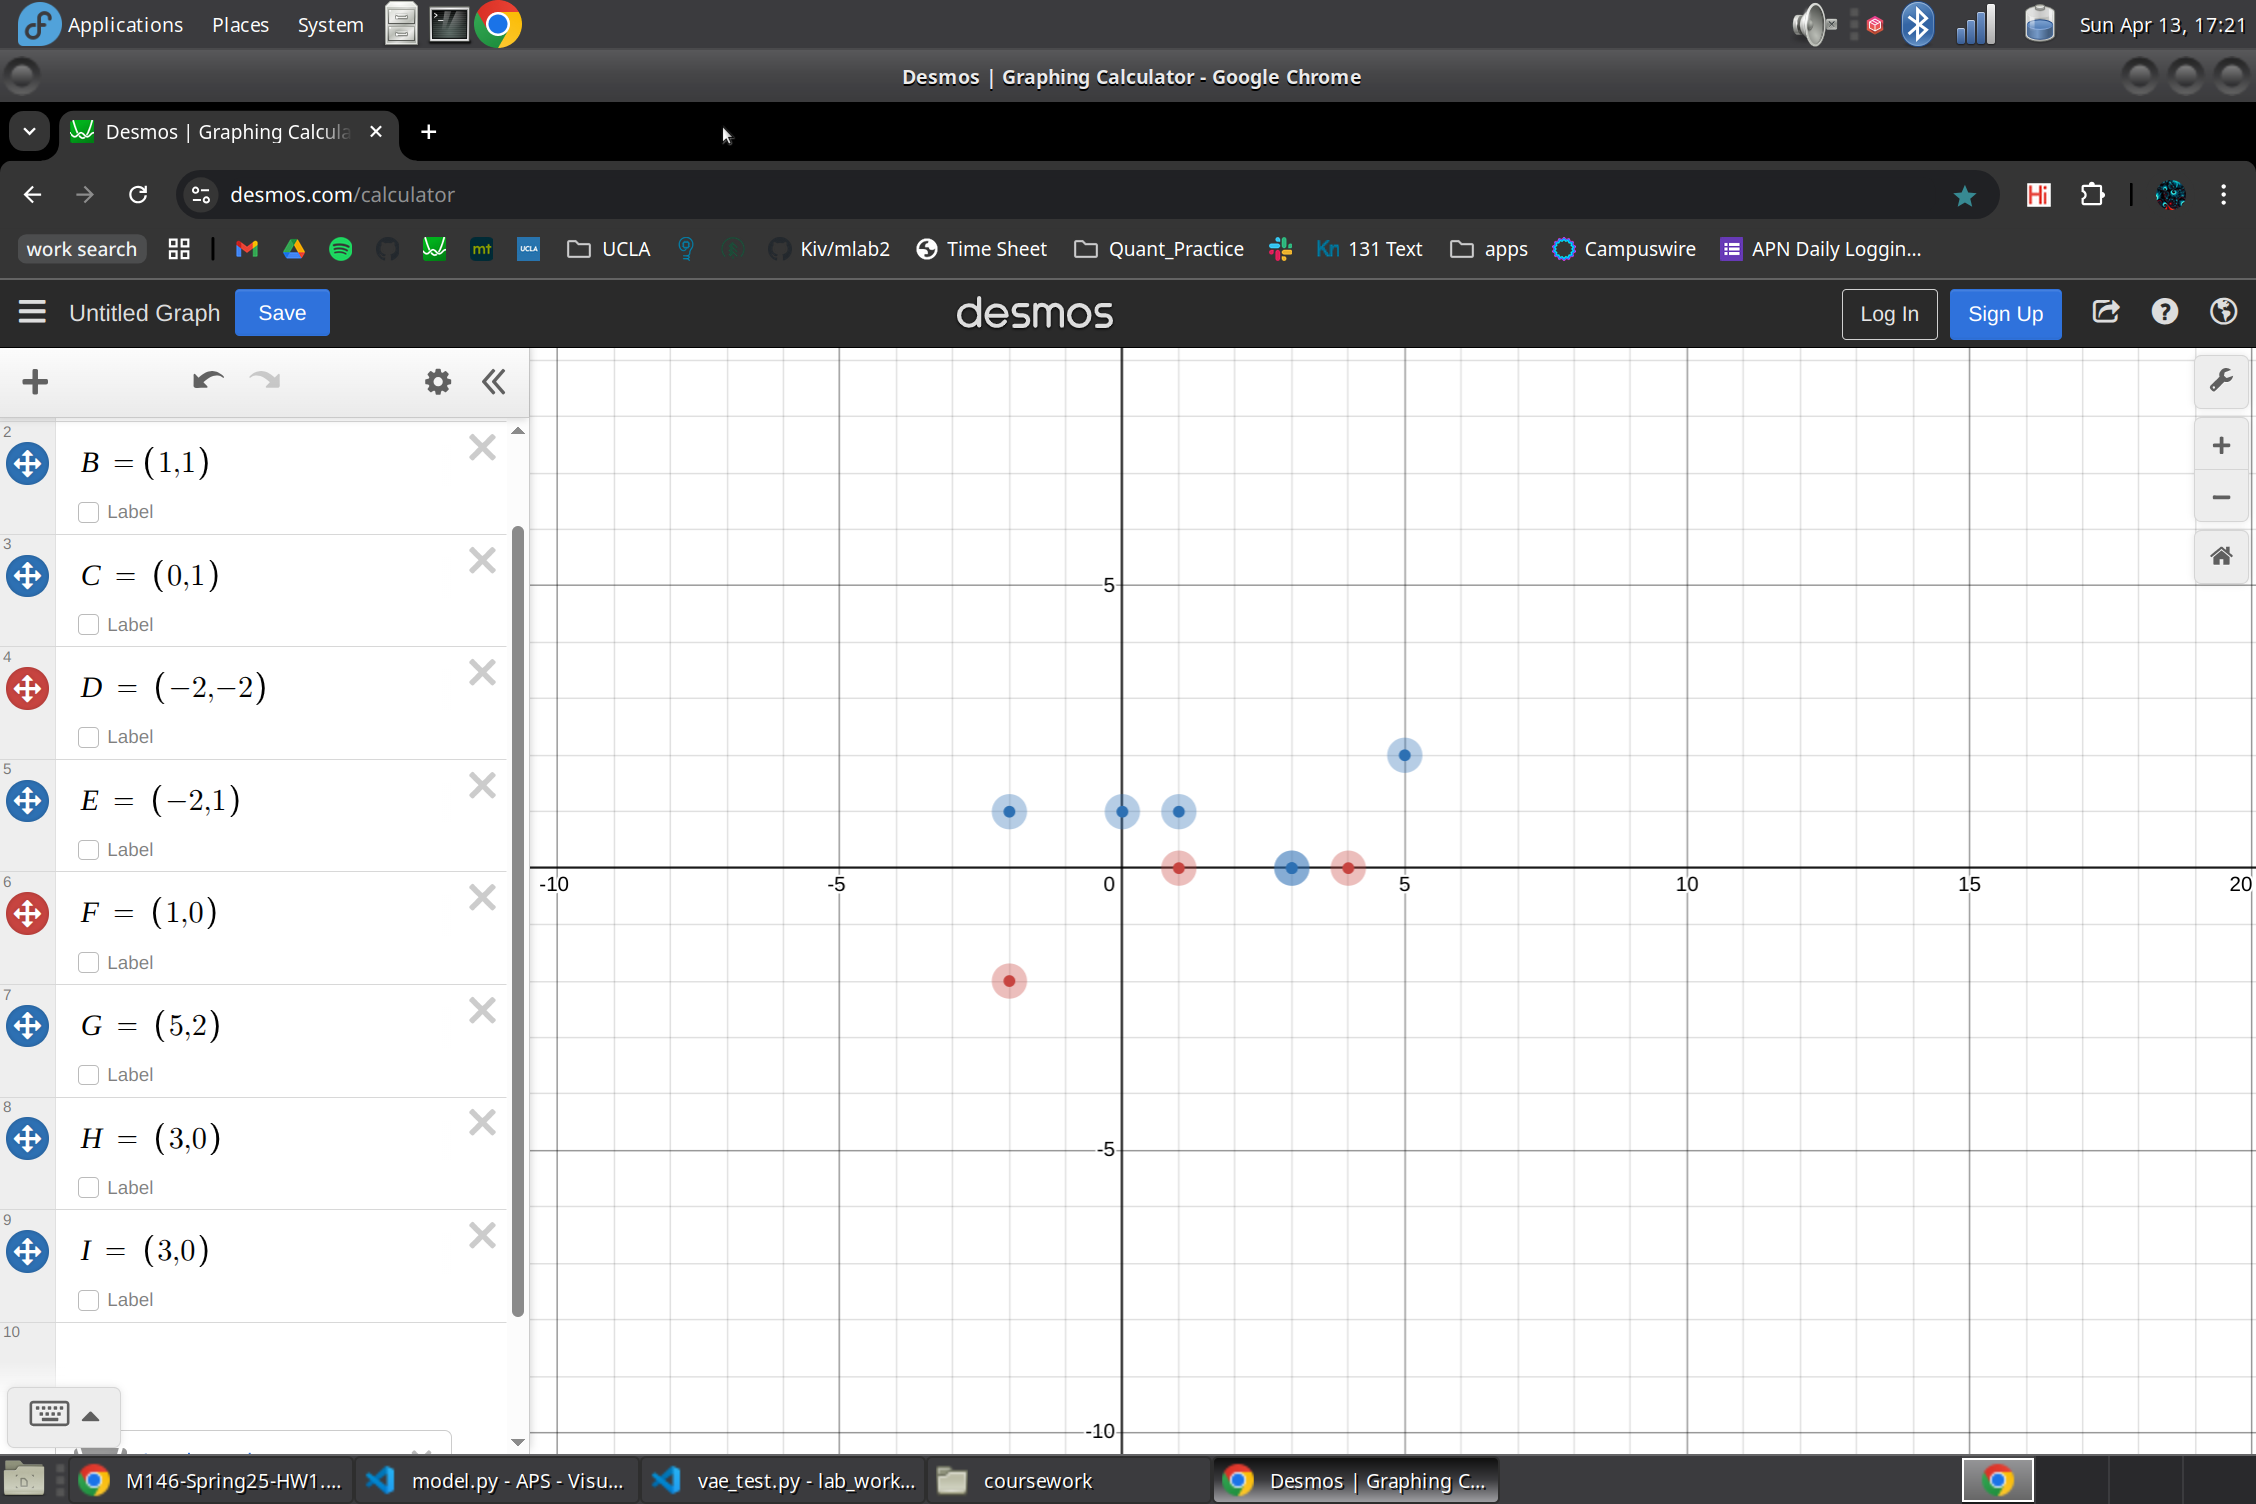
\includegraphics[width=\textwidth]{q1.png}. Any linear classifier must pass through the origin since there is no bias. Additionally the line created by the classifier
            must have positive slope to correctly classify the point at (1,0), yet this will cause it to incorrectly classify the point at (3,0)
        \item $w_1 = x_1 = \begin{pmatrix} 4 \\ 0 \end{pmatrix} $, $m=1$, $s_1 = 1$
            \begin{align*}
                w_1^{T}x_1 &= 16 > 0\\
                s_1 &= s_1 + 1 = 2\\
                w_1^{T}x_2 &= 4 > 0\\
                w_2 &\leftarrow w_1 - x_2 = \begin{pmatrix} 3 \\ -1 \end{pmatrix} \\
                m &= m + 1 = 2, s_2 = 1\\
                w_2^{T}x_3 &= -1 < 0\\
                s_2 &= s_2 + 1 = 2\\
                w_2^{T}x_4 &= -4 < 0\\
                w_3 &\leftarrow w_2  + x_4 = \begin{pmatrix} 1 \\ -3 \end{pmatrix} \\
                m &= m + 1 = 3, s_3 = 1\\
                w_3^{T}x_5 &= -5 < 0\\
                s_3 &= s_3 + 1 = 2\\
                w_3^{T}x_6 &= 1 > 0\\
                s_3 &= s_3 + 1 = 3\\
                w_3^{T}x_7 &= -1 < 0\\
                s_3 &= s_3 + 1 = 4\\
                w_3^{T}x_8 &= 3 > 0\\
                w_4 &\leftarrow w_3 - x_8 = \begin{pmatrix} -2 \\ -3 \end{pmatrix} \\
                m &= m +1 = 4, s_4 = 1
            \end{align*}
        \item 
            \begin{enumerate}
                \item For regular perceptron:\\
                    \[
                    \hat y = 
                    \begin{cases}
                        1 & \begin{pmatrix} -2 \\ -3 \end{pmatrix}^{T} \hat x \ge 0\\
                        -1 & \begin{pmatrix} -2 \\ -3 \end{pmatrix}^{T} \hat x < 0
                    \end{cases}
                    = \text{sign}(\begin{pmatrix} -2 \\ -3 \end{pmatrix}^{T}x)
                    .\] 
                \item For voted perceptron
                    \[
                        \hat y = \text{sign}[2\text{sign}(\begin{pmatrix} 4 \\ 0 \end{pmatrix}^{T}x) + 2\text{sign}(\begin{pmatrix} 3 \\ -1 \end{pmatrix}^{T}x) + 4\text{sign}(\begin{pmatrix} 1 \\ -3 \end{pmatrix}^{T}x) + \text{sign}(\begin{pmatrix} -2 \\ -3 \end{pmatrix}^{T}x)]
                    .\] 
                \item For average perceptron
                    \[
                        \hat y = \text{sign}[2(\begin{pmatrix} 4 \\ 0 \end{pmatrix}^{T}x) + 2(\begin{pmatrix} 3 \\ -1 \end{pmatrix}^{T}x) + (\begin{pmatrix} 1 \\ -3 \end{pmatrix}^{T}x) + (\begin{pmatrix} -2 \\ -3 \end{pmatrix}^{T}x)]
                    .\] 
            \end{enumerate}
        \item 
            \begin{enumerate}
                \item For regular perceptron error:\\
                    \begin{align*}
                        w_4^{T}x_1 = -8 &\hspace{1cm} \text{incorrect}\\
                        w_4^{T}x_2 = -5 &\hspace{1cm} \text{correct}\\
                        w_4^{T}x_3 = -3 &\hspace{1cm} \text{correct}\\
                        w_4^{T}x_4 = 10 &\hspace{1cm} \text{correct}\\
                        w_4^{T}x_5 = 1 &\hspace{1cm} \text{incorrect}\\
                        w_4^{T}x_6 = -2 &\hspace{1cm} \text{incorrect}\\
                        w_4^{T}x_7 = -16 &\hspace{1cm} \text{correct}\\
                        w_4^{T}x_8 = -6 &\hspace{1cm} \text{correct}
                    \end{align*}
                    accuracy $\frac{5}{8} = 62.5\%$
                \item For voted perceptron error:
                    \begin{align*}
                        \hat y_1 = 1 &\hspace{1cm} \text{correct}\\                        
                        \hat y_2 = -1 &\hspace{1cm} \text{correct}\\                        
                        \hat y_3 = -1 &\hspace{1cm} \text{correct}\\                        
                        \hat y_4 = 1 &\hspace{1cm} \text{correct}\\                        
                        \hat y_5 = -1 &\hspace{1cm} \text{correct}\\                        
                        \hat y_6 = 1 &\hspace{1cm} \text{correct}\\                        
                        \hat y_7 = -1 &\hspace{1cm} \text{correct}\\                        
                        \hat y_8 = 1 &\hspace{1cm} \text{incorrect}\\                        
                    \end{align*}
                    for total accuracy $\frac{7}{8} = 87.5\%$
                \item For average perceptron error:
                    \begin{align*}
                        \hat y_1 = 1 &\hspace{1cm} \text{correct}\\                        
                        \hat y_2 = -1 &\hspace{1cm} \text{correct}\\                        
                        \hat y_3 = -1 &\hspace{1cm} \text{correct}\\                        
                        \hat y_4 = 1 &\hspace{1cm} \text{correct}\\                        
                        \hat y_5 = -1 &\hspace{1cm} \text{correct}\\                        
                        \hat y_6 = 1 &\hspace{1cm} \text{correct}\\                        
                        \hat y_7 = 1 &\hspace{1cm} \text{incorrect}\\                        
                        \hat y_8 = 1 &\hspace{1cm} \text{incorrect}\\                        
                    \end{align*}
                    for total accuracy $\frac{6}{8} = 75\%$
            \end{enumerate}

    \end{enumerate}
}
\section{Problem 2}
\solution{
    \[
        J(w_0,w_1) = \sum_{n=1}^{N}\alpha_n(w_0 + w_1x_{n,1}-y_n)^2
    .\] 
    implies
    \[
        \frac{\partial J}{\partial w_0} = 2\sum_{n=1}^{N}\alpha_n(w_0+w_1x_{n,1}-y_n)
    .\] 
    and
    \[
        \frac{\partial J}{\partial w_1} = 2\sum_{n=1}^{N}\alpha_n(w_0+w_1x_{n,1}-y_n)x_{n,1}
    .\] 
    \[
        \frac{\partial^2 J}{\partial w_0^2} = 2 \sum_{n=1}^{N}\alpha_n
    .\] 
    \[
        \frac{\partial^2 J}{\partial w_0 \partial w_1} = \frac{\partial^2 J}{\partial w_1 \partial w_0} = 2\sum_{n=1}^{N}\alpha_nx_{n,1}
    .\] 
    \[
        \frac{\partial^2 J}{\partial w_1^2} = 2\sum_{n=1}^{N}\alpha_n x_{n,1}^2
    .\] 
    \[
    H = \begin{pmatrix} 
        2\sum_{n=1}^{N}\alpha_n & 2\sum_{n=1}^{N}\alpha_nx_{n,1}\\
        2\sum_{n=1}^{N}\alpha_nx_{n,1} & 2\sum_{n=1}^{N}\alpha_nx_{n,1}^2
    \end{pmatrix} 
    .\] 
    \[
        z^{T}Hz = \begin{pmatrix} 2z_1\sum_{n=1}^{N}\alpha_n + 2z_2\sum_{n=1}^{N}\alpha_nx_{n,1} & 2z_1\sum_{n=1}^{N}\alpha_nx_{n,1} + 2z_2\sum_{n=1}^{N}\alpha_nx_{n,1}^2 \end{pmatrix} 
    .\] 
    \[
        = 2\sum_{n=1}^{N}\alpha_nz_1^2 + \alpha_nx_{n,1}z_1z_2 + z_1z_2\alpha_nx_{n,1} + z_2^2\alpha_nx_{n,1}^2
    .\] 
    \[
        2\sum_{n=1}^{N}\alpha_n(z_1^2 + 2z_1z_2x_{n,1} + z_2^2x_{n,1}^2) = 2\sum_{n=1}^{N}\alpha_n(z_1+z_2x_{n,1})^2 \ge 0
    .\] 
    so the hessian is PSD and $J(w_0,w_1)$ is convex, thus there exists a global optimum
}

\section{Problem 3}
\solution{
    \begin{enumerate}
        \item 
            \[
            h_w(x) = \frac{e^{w^{T}x}}{1 + e^{w^{T}x}}
            .\] 
            \[
                \tanh_w(x) = \frac{e^{2w^{T}x} - 1}{e^{2w^{T}x}+1}
            .\] 
            consider
            \[
            2h_{2w}(x) - 1 = \frac{2e^{2w^{T}x}}{1 + e^{2w^{T}x}} - \frac{1 + e^{2w^{T}x}}{1 + e^{2w^{T}x}} = \frac{e^{2w^{T}x}-1}{e^{2w^{T}x} + 1} = \tanh_w(x)
            .\] 
        \item 
            \[
            \lim_{x\to +\infty} \frac{\left(e^{2x}-1\right)}{e^{2x}+1} = 1
            .\] 
            \[
            \lim_{x\to -\infty} \frac{\left(e^{2x}-1\right)}{e^{2x}+1} = -1
            .\] 
            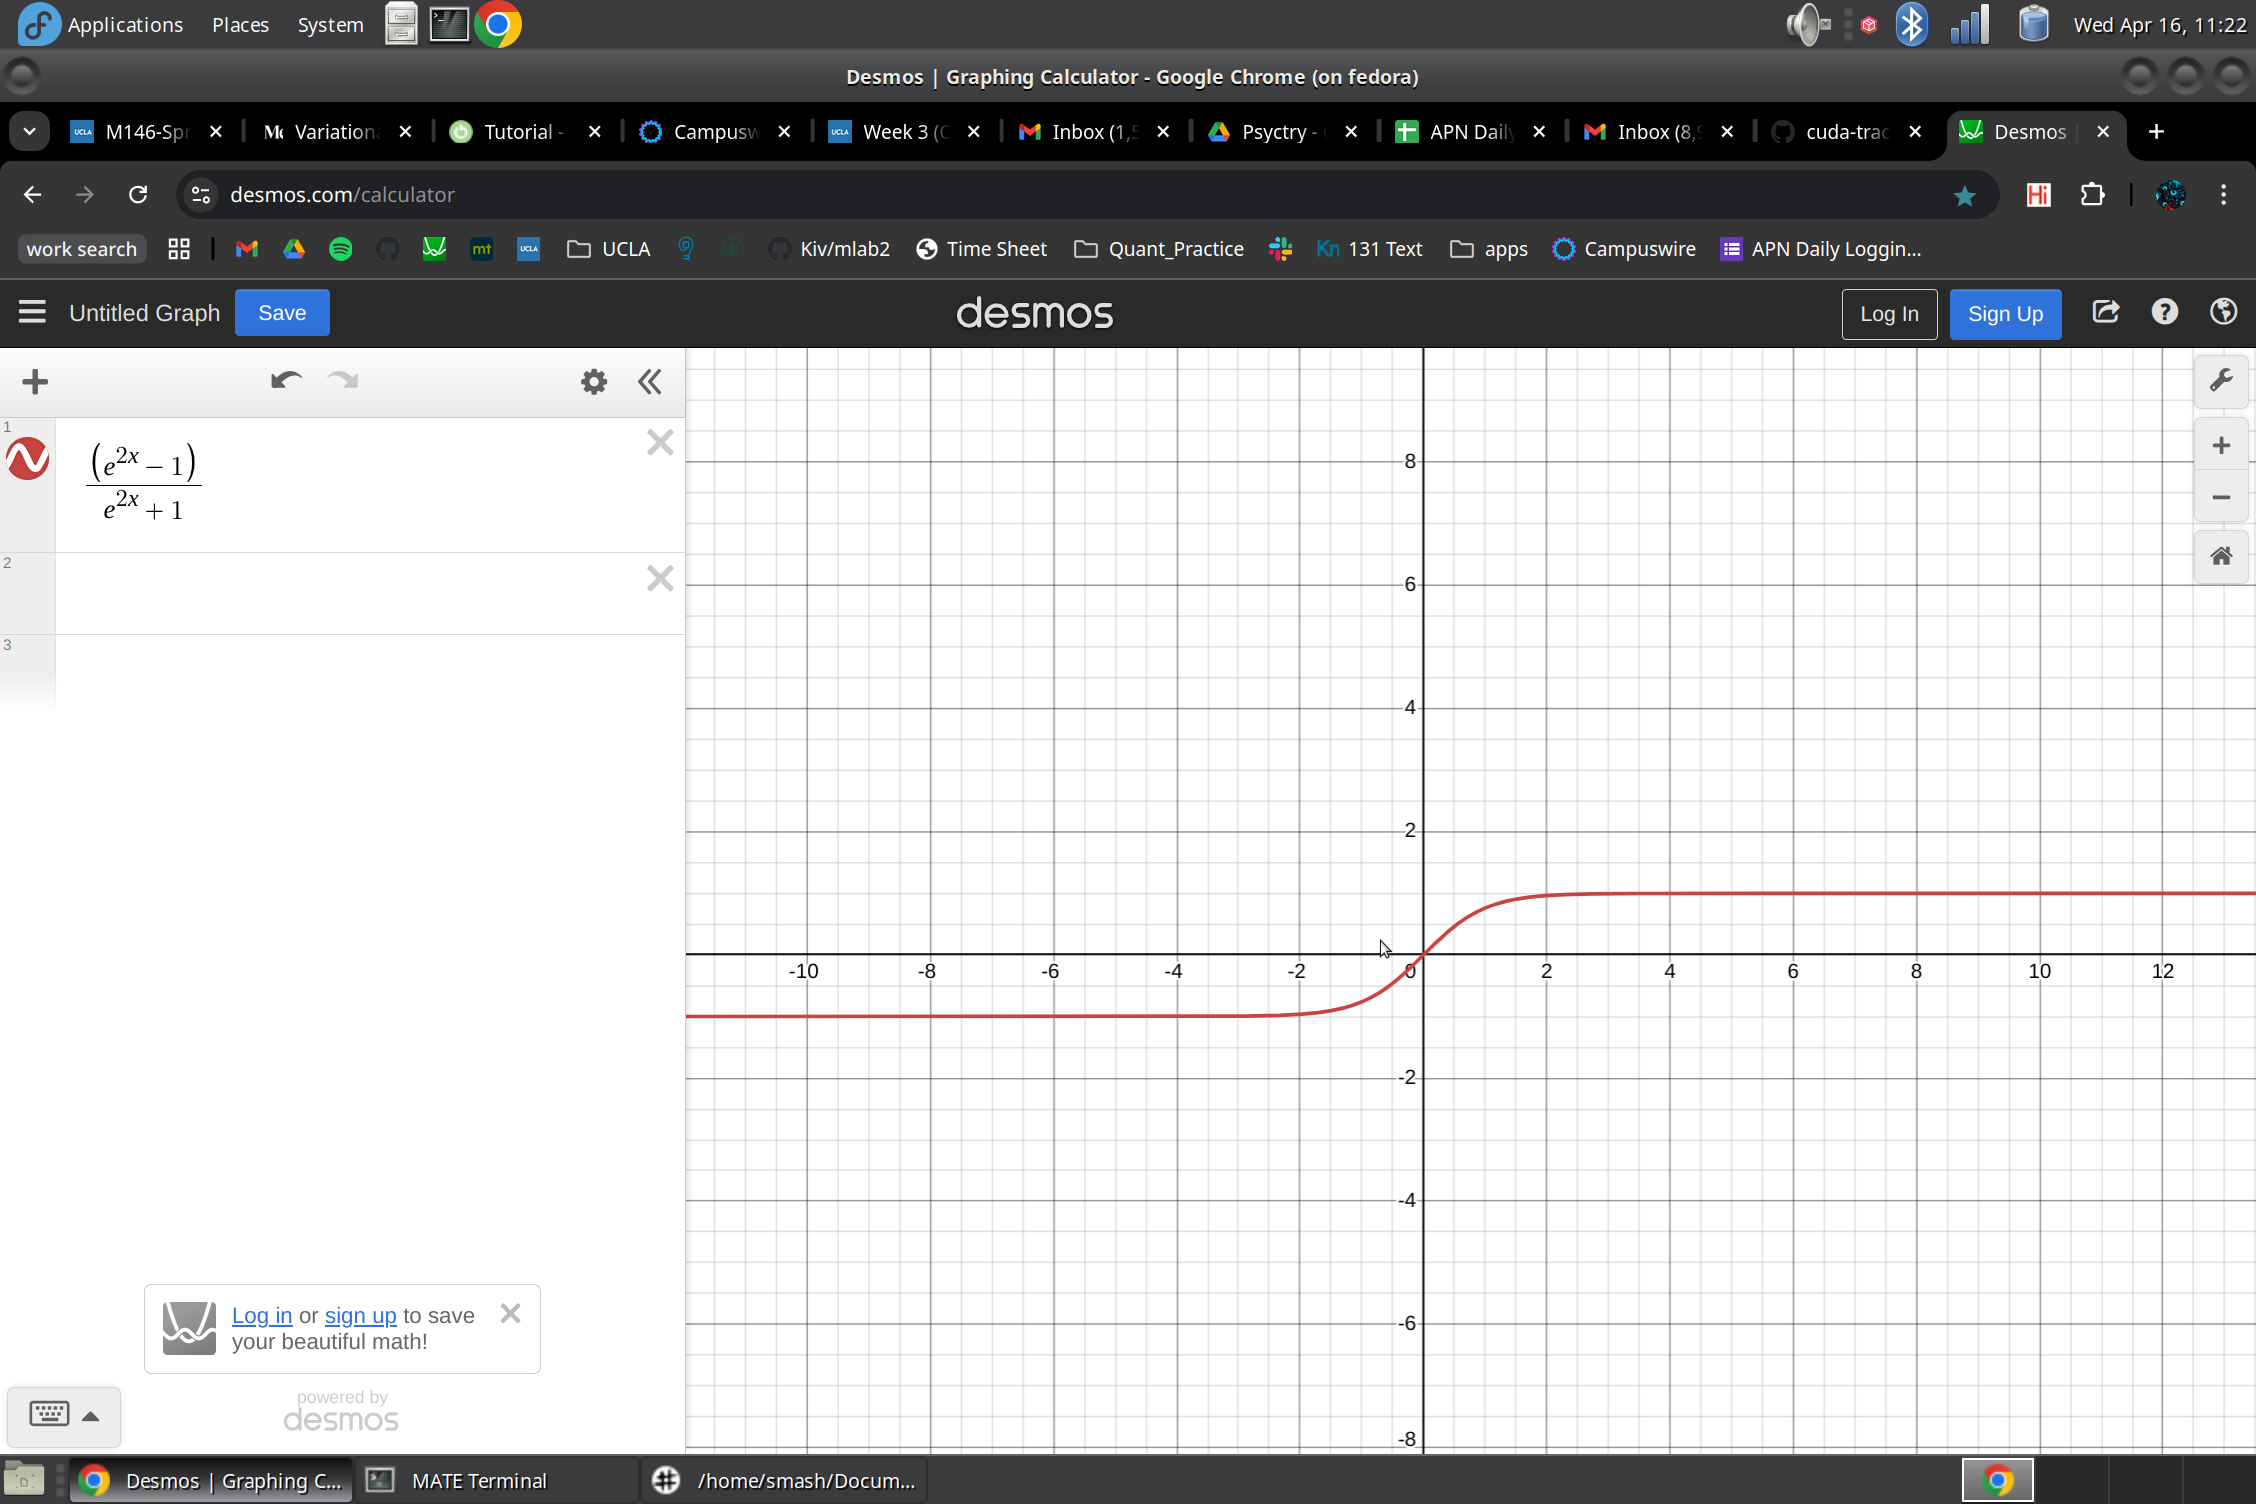
\includegraphics[width = \textwidth]{tanh.png} You can use the criterion, $\tanh_w(x) \ge 0$ to decide on the label $+1$ and $\tanh_w(x) < 0$ for $-1$
        \item Since $\tanh$ can output negative values $\log(\tanh_w(x_i))$ can be undefined.
        \item Define the bijection of $\hat y_i \rightarrow  y_i$ by
            \[
            y_i = 
            \begin{cases}
                1 & \hat y_i = 1\\
                0 & \hat y_i = -1
            \end{cases}
             =  \frac{1 + \hat y_i}{2}
            .\] 
            then
            \[
                (1-y_i) = \frac{1-\hat y_i}{2}
            .\] 
            and since rearranging the previous equation we get
            \[
                h_{w'}(x_i) = \frac{1 + \tanh_{w}(x_i)}{2}
            .\] 
            \[
                1 - h_{w'}(x_i) = \frac{1-\tanh_w(x_i)}{2}
            .\] 
            and so plugging these in we get the optimization problem is equivalent to
            \[
                \min_{w} - \sum_{i=1}^{n}[\frac{1+\hat y_i}{2}\log(\frac{1 + \tanh_w(x_i)}{2}) + \frac{1-\hat y_i}{2}\log( \frac{1-\tanh_w(x_i)}{2})]
            .\] 
            for any $x_i$ if $\hat y_i = 1$ then the contribution to the loss is
             \[
            l(w,x_i) = \log(\frac{1 + \tanh_w(x_i)}{2})
            .\] 
            the gradient is
            \[
                \frac{\partial l}{\partial w} = \frac{1}{(1 + \tanh_w(x_i))} \frac{\partial}{\partial w}(\tanh_w(x_i))
            .\] 
            \[
            \frac{\partial}{\partial w} \tanh_w(x_i) = (-\tanh_w^2(x_i) + 1)x_i = x_i(1+\tanh_w(x_i))(1-\tanh_w(x_i))
            .\] 
            so the gradient is
            \[
                \frac{\partial l}{\partial w} = x_i(1-\tanh_w(x_i))
            .\] 
            if instead $\hat y_i = -1$ the only contribution to the loss is
             \[
            l(w,x_i) = \log(\frac{1-\tanh_w(x_i)}{2})
            .\] 
            \[
                \frac{\partial l}{\partial w} = -\frac{1}{1- \tanh_w(x_i))} \frac{\partial}{\partial w} (\tanh_w(x_i))
            .\] 
            so the gradient is
            \[
            -x_i(1+\tanh_w(x_i))
            .\] 
    \end{enumerate}
}
\section{Problem 4}
\solution{
    \begin{enumerate}
        \item Visualization
            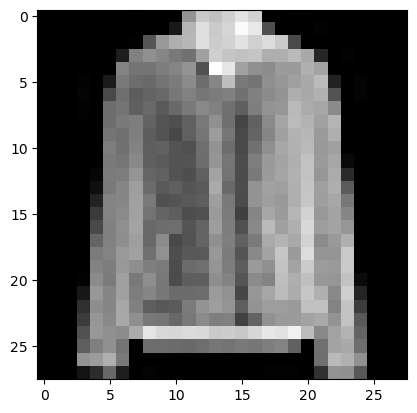
\includegraphics[width=5cm]{q4.png}
            $X_{\text{train}}.\text{shape} = (5000, 784)$\\
            $X_{\text{test}}.\text{shape} = (500, 784)$
    \end{enumerate}
}

\end{document}
